In order to probe the various aspects of the well-established standard model or search for hints of new physics beyond the SM, particle physics experiments preferentially make use of powerful particle accelerators where particles of a certain type are collided in order to probe the constituents of matter and interactions between them. The analyses presented in this thesis are all performed in the context of the CMS experiment located at the Large Hadron Collider (LHC) at CERN near Geneva. \\ 
The first part of this chapter provides an introduction to the LHC. This is followed by an overview of the detector system of the CMS experiment. Afterwards the hitherto periods of collision data taking at the LHC are discussed together with an introduction to the generation of simulated events which are used in the analysis of real data events.  
\section{The Large Hadron Collider}
\label{sec:lhc}
The Large Hadron Collider~\cite{Bruning:782076, 1748-0221-3-08-S08001} is a ring-accelerator designed to provide particle collisions of hadrons. It is built in the tunnel of the former LEP~\cite{LEPdesign} collider 45 -- 170\,m below the ground and has a circumference of 26.7\,km. The LHC is a particle-particle collider and thus composed of two rings with counter-rotating beams. The operation can be performed in different modes with either proton beams or heavy ions like e.g. lead~\footnote{All studies presented in this thesis are based on proton-proton collisions. Thus the operation with heavy ions is not discussed.}. \\
In each beam, protons are grouped together in bunches and accelerated in two evacuated beam pipes using superconducting radio-frequency cavities. With a nominal bunch spacing of 25\,ns the bunch revolution frequency is 40\,MHz. Each of the 2808 individual bunches per beam contains at design conditions $1.15 \times 10^{11}$ protons. In order to bend the beams around the LHC ring superconducting dipole magnets are used with an operation temperature of 1.9\,K. They provide a magnetic field of up to 8.33\,T while additional quadrupole and sextupole magnets are utilized to squeeze and focus the beams.\\  
Before the protons are injected into the LHC they are already pre-accelerated in various smaller accelerators up to a beam energy of 450\,GeV while passing through the injector chain Linac2 -- Proton Synchrotron Booster (PSB) -- Proton Synchrotron (PS) -- Super Proton Synchrotron (SPS). An overview of the accelerator complex at CERN is given in Fig.~\ref{fig:AccComplex}.
\begin{figure}[!tp]
  \centering
  \begin{tabular}{c}
    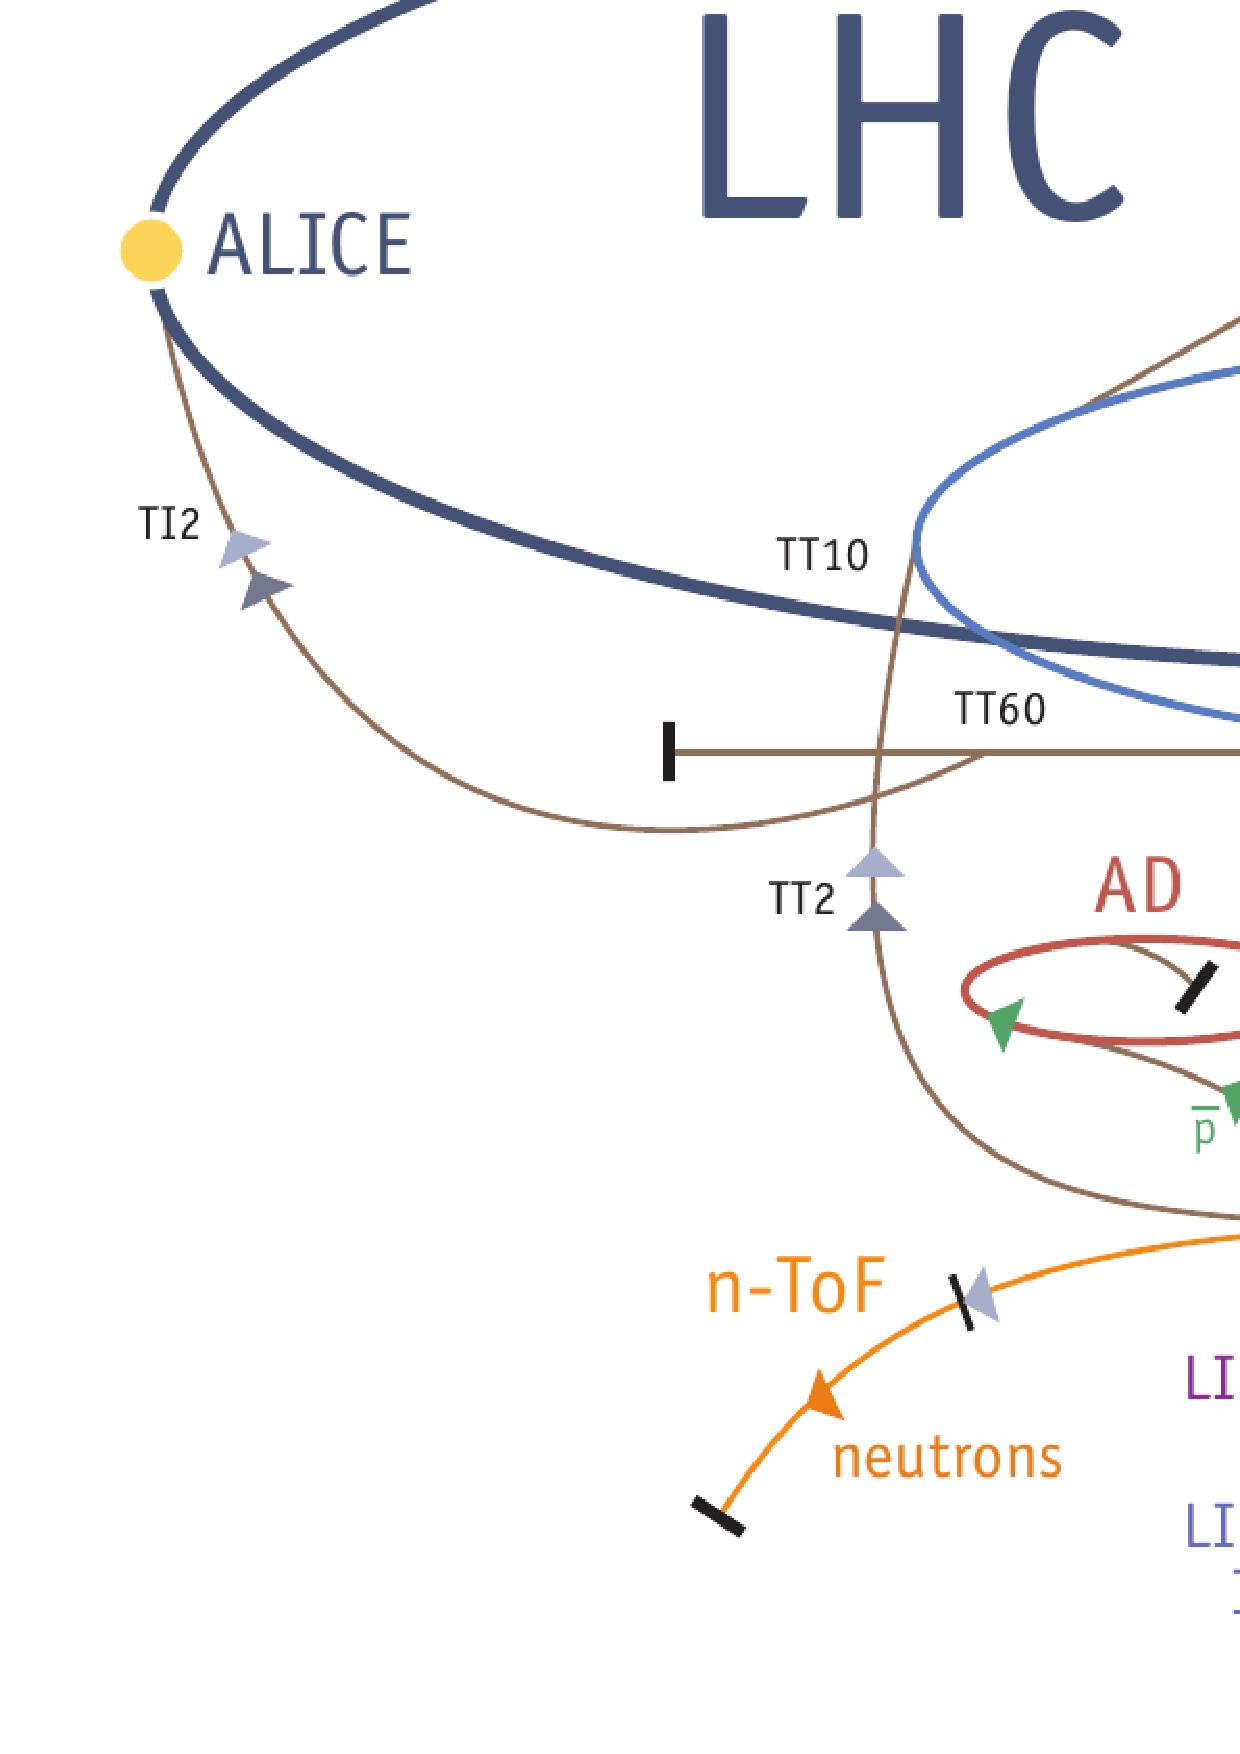
\includegraphics[width=0.9\textwidth]{figures/lhc.jpg}
  \end{tabular}
  \caption{Illustration of the CERN accelerator complex including the injector chain of the LHC ring. Taken from~\cite{CERNaccelerators}.}
  \label{fig:AccComplex}
\end{figure}
\\
\\
The main goal of the LHC is to provide proton-proton collisions to the experiments with center of mass energies up to 14\,TeV in order to explore physics processes at novel energy regimes. The expected number of events $N$ for a certain type of process is given by the product of the specific cross section $\sigma$ of that process and the integral $L = \int \mathcal{L}  \, dt$ of the instantaneous luminosity $\cal L$ over time such that
\begin{equation}
  N = \sigma \cdot L . 
  \label{eq:lumi}
\end{equation}
The luminosity is a machine parameter and can be expressed for beams with Gaussian-shaped profiles as  
\begin{equation}
  \mathcal{L} = \frac{f n_{1} n_{2}}{4 \pi \sigma_{x} \sigma{y}} \cdot F
  \label{eq:lumi}
\end{equation}
with the revolution frequency $f$, the number of particles $n_1$ and $n_2$ contained in the two colliding bunches and the transverse beam sizes $\sigma_{x}$ ($\sigma_{y}$) in the horizontal (vertical) directions. In order to take the inclination of the two beams into account, the geomatrical correction factor $F$ is introduced. The nominal peak luminosity of the LHC is $10^{34} \, \mathrm{cm}^{-2} \, \mathrm{s}^{-1}$. Since the total inelastic proton-proton cross-section at a center of mass energy of 14~TeV is close to 100\,mb as indicated in Fig.~\ref{fig:CrossSections}, the expected event rate is approximately $10^9$ events per second. This is resulting in high technical challenges for the experiments. \\
\begin{figure}[!tp]
  \centering
  \begin{tabular}{c}
    \includegraphics[width=0.60\textwidth]{figures/crosssections2012_v5-1.pdf}
  \end{tabular}
  \caption{Summary of cross sections for various standard model processes in proton-proton and proton-antiproton collisions as function of the centre of mass energy. The right axis displays the correponding event rate at a luminosity of $\mathrm{10^{33}\,cm^{-2} s^{-1}}$. Taken from~\cite{bib:stirling:pcom}.}
  \label{fig:CrossSections}
\end{figure}
\\
The four main experiments are located at the four locations along the LHC ring where the beams cross in order to measure the delivered particle collisions. The two high luminosity experiments ATLAS~\cite{det::ATLAS} and CMS~\cite{Chatrchyan:2008zzk, bib:cmsptdr1} are designed for multiple purposes like precision measurements of SM quantities, search for the standard model Higgs Boson or searches for signals indicating new physics processes. The LHCb detector~\cite{det::LHCb} however is a specialised experiment focusing on the measurement of CP violation in the interactions of hadrons containing b-quarks. The only experiment designed especially for the analysis of heavy ion collisions is the ALICE~\cite{det::ALICE} detector with the main emphasis on the physics of strongly interacting matter at extreme energy densities like for instance quark-gluon plasma.

\section{The CMS Experiment}
\label{sec:cms}
The CMS detector is one of the two experiments at the LHC designed to address a multitude of physics questions. In addition to tests of the SM at the TeV scale, studies of the nature of elektroweak symmetry breaking which might show up in the presence of a Higgs boson and searches for so far unknown particles pointing to e.g. new symmetries in nature are the primary targets of these experiments. These ambitious physics goals can only be achieved by fully exploiting the by now unprecedented collision energy and luminosity.\\
\\
The CMS detector with its typical cylindrical design of different sub-detector components around the beam line is designed to perfectly meet these particular conditions. A sketch of the CMS detector and the different sub-detectors is shown in Fig.~\ref{fig:CMS}.
\begin{figure}[!tp]
  \centering
  \begin{tabular}{c}
    \includegraphics[width=1.0\textwidth]{figures/Figures_Experimental_Apparatus_CMS_perspective.png}
  \end{tabular}
  \caption{A perspective view of the CMS detector~\cite{Chatrchyan:2008zzk}.}
  \label{fig:CMS}
\end{figure}
As a typical high-energy particle experiment the CMS detector makes mainly use of tracking detectors and calorimeters to measure particles' momenta, energy depositions and flight directions in order to identify the objects emerging from the particle collisions. The entire CMS detector with a length of 21.6\,m and a diameter of 14.6\,m results in a total weight of 12500\,t. \\  
The following sections comprise a description of the CMS detector and individual sub-detector components focusing on the detector parts most relevant for the analyses presented in this thesis. A detailed discussion of the detector design can be found in~\cite{Chatrchyan:2008zzk, bib:cmsptdr1}.

\subsection{Coordinate Conventions and Kinematic Variables}
\label{subsec:cms_coordinates}
In order to describe the particle collisions, the CMS experiment makes use of a right-handed coordinate system with its origin at the center of the detector at the nominal interaction point. While the z-axis is defined along the direction of the beam, the x-axis points to the center of the LHC ring and the y-axis vertically upwards. In this xy-plane the azimuthal angle $\phi$ is measured where $\phi = 0$ coincides with the x-axis. The polar angle $\theta$ however is defined with respect to the z-axis. A quantity closely related to the polar angle is the pseudorapidity $\eta$ defined as
\begin{equation}
\eta = \mathrm{-ln} \left[\mathrm{tan} \left(\frac{\theta}{2} \right)\right]
\end{equation}
which is widely used in experimental particle physics as rapidity differences are Lorentz invariant. A pseudorapidity $\eta = 0$ corresponds to the direction perpendicular to the beam while $|\eta| \rightarrow \infty$ points along the beam. Based on the pseudorapidity the Lorentz invariant distance between two objects $\Delta$R can be written as
\begin{equation}
\Delta \mathrm{R} = \sqrt{(\Delta \eta)^2 + (\Delta \phi)^2} \, .
\end{equation}
At the LHC the initial conditions of the primary collisions are not known as the specific energy fraction of the proton which each parton carries can not be identified. Thus conservation of the total momentum can not be utilized directly to describe the momentum balance in the final state. However, it is known that the initial particles have no significant momentum orthogonal to the beam axis which is referred to as transverse momentum 
\begin{equation}
\pt = p \cdot \mathrm{sin}\theta \, .
\end{equation}
Thus, momentum conservation in the transverse plane is used to describe the final state conditions. Any difference between the total sum of all transverse momenta and zero is considered as missing energy \met and often exploited to describe undetected particles.

\subsection{Superconducting Magnet}
\label{subsec:cms_magnet}
The CMS experiment makes use of a large superconducting solenoid magnet which is a crucial component of the whole detector design and provides a magnetic field of up to 4\,T. It allows to precisely determine the momenta and charge of charged particles from the bended tracks that they follow in the magnetic field.\\
With a length of 12.5\,m and a diameter of the free bore of 6.3\,m the total cold mass reaches 220\,t. It is made up of a niobium-titanium coil which is winded in 4-layers. This configuration allows a storage of 2.6\,GJ energy at full current. A 10000\,t heavy-weight iron yoke is responsible for the return of the magnetic flux.

\subsection{Inner Tracking System}
\label{subsec:cms_tracker}
The tracking system of the CMS experiment is the innermost part of the detector and installed directly around the interaction point completely contained in the bore of the magnet system. Its' purpose is to precisely measure the trajectories of charged particles arising from the collisions as well as to reconstruct secondary vertices. Due to the location close to the interaction point the tracking system has to cope with a high particle flux crossing the tracker associated with each bunch crossing. Hence high requirements on response time and granularity are set in order to properly identify the particles' tracks. \\
In order to fulfill these tasks the CMS experiment makes use of a tracker design based on silicon detectors. It consists of mainly two components: the innermost part is made of silicon pixel detectors while these are surrounded by silicon strip modules. In total they add up to an active area of 200\,$\mathrm{m}^2$ with a length of 5.8\,m and a diameter of 2.5\,m covering the detector up to $|\eta| = 2.5$. A schematic overview of the whole tracking system is shown in Fig.~\ref{fig:CMS_tracker}. 
\begin{figure}[!tp]
  \centering
  \begin{tabular}{c}
    \includegraphics[width=0.9\textwidth]{figures/Figures_Experimental_Apparatus_Tracker.png}
  \end{tabular}
  \caption{Sketch of the CMS tracking system in a $rz$-view. Each tracker module is represented by one line. Taken from~\cite{Chatrchyan:2008zzk}.}
  \label{fig:CMS_tracker}
\end{figure}
\begin{description}
 \item \textbf{Pixel Detector:} The pixel detector consists of three barrel layers which extend from 4.4\,cm to 10.2\,cm and two endcap disks on each side. In total there are 1440 pixel modules installed. The size of one pixel cell is 100 x 150 $\mu m^2$ providing similar track resolution quality in $r-\phi$ and $z$ direction. This configuration provides for almost the whole range up to $|\eta| = 2.5$ three precise tracking hits. This is especially important for the reconstruction of secondary vertices.
 \item \textbf{Silicon Strip Tracker:} The silicon strip detector which extends to a radius of 1.1\,m comprises the pixel tracker. The more than 15000 individual strip detector modules are arranged in an inner and an outer detector part. The inner part of the strip tracker is build by the four Tracker Inner Barrel (TIB) layers which are accompanied by the three Tracker Inner Disks (TID) at the end sides. This inner part provides up to four track measurements in the $r-\phi$ plane. The TIB/TID system lies within the Tracker Outer Barrel (TOB) consisting of another six barrel layers while it is complemented by the Tracker EndCaps (TEC) which add another nine disks at each side of the tracking system. This layout provides at least around nine hits within the silicon strip system. 
\end{description}
The tracking system with the desgin described above provides a very good impact parameter resolution and tracking efficiency~\cite{bib:cmstdr:tracker}. The impact parameter resolution is of the order of $<$ 35\,$\mu$m in the plane perpendicular to the beam (for particles with \pt $>$ 10\,GeV) and reaches 75\,$\mu$m in the longitudinal direction. Also the track reconstruction efficiency is expected to show a very good performance. The track reconstruction efficiency of high energetic electrons is above 90\%, that of charged hadrons up to 95\% (for \pt $>$ 10\,GeV) and that for muons even better than 98\% in the whole covered region up to $|\eta| = 2.5$ already for muons with very low transverse momenta around 1\,GeV. Altogether, the relative transverse momentum resolution reaches a level of 1-2\% for high momentum tracks ($\approx$ 100\,GeV) in the central barrel for $|\eta| < 1.6$.
 

\subsection{Electromagnetic Calorimeter}
\label{subsec:cms_ecal}
The CMS experiment makes use of a homogeneous electromagnetic calorimeter (ECAL) in order to precisely measure the energy deposits of electrons and photons. It is installed around the inner tracking system covering a range up to $|\eta| = 3.0$ and consists of lead tungstate (PbW$\mathrm{O}_4$) crystals. These have been chosen as they provide a high density, short radiation length and a small Moli\`{e}re radius and hence allow to build a compact calorimeter with a fine granularity. As 80\% of the scintillation light is emitted within 25\,ns, this matches well the bunch crossing rate of the LHC machine. In order to collect the radiated light photodiodes are glued to the back of each crystal. \\
An overview of the ECAL layout is shown in Fig.~\ref{fig:CMS_ecal}. The individual sub-components are the following:
\begin{figure}[!tp]
  \centering
  \begin{tabular}{c}
    \includegraphics[width=0.9\textwidth]{figures/Figures_Experimental_Apparatus_ECALRapidity.png}
  \end{tabular}
  \caption{View of one quarter section of the CMS electromagnetic calorimeter in a yz-view. Taken from~\cite{bib:cmsptdr1}.}
  \label{fig:CMS_ecal}
\end{figure}
\begin{description}
 \item \textbf{Barrel ECAL (EB):} The barrel detector of the ECAL covers the pseudorapidity region up to $|\eta| = 1.479$. Within a radius of about 1.3\,m a total number of 61200 crystals are installed. Each of them has a length of 230\,mm resulting in a radiation length of 25.8 $\mathrm{X_0}$. The crystal cross-section in $(\eta, \phi)$ is $(0.0174, 0.0174)$. Avalanche photodiodes are used to detect the emitted scintillation light.
 \item \textbf{Endcap ECAL (EE):} The EB is complemented on each side by an endcap which consists of two d-shaped halfs. The ECAL endcaps extend from $|\eta| = 1.479$ to $|\eta| = 3.0$. In total they contain another 14648 crystals with an individual length of 220\,mm corresponding to 24.7 $\mathrm{X}_0$. For the collection of scintillation light vacuum phototriodes are used in the endcaps.
 \item \textbf{Preshower (ES):} In front of the endcap crystals a preshower detector is placed. It covers the pseudorapidity range of $|\eta| = 1.653 - 2.6$. The main purpose is to identify photons emerging from the decay of neutral pions. It is a two-layer sampling calorimeter with lead as absorber material and silicon strip sensors measuring the deposited energy. The total thickness of the preshower is 20\,cm (3 $\mathrm{X_0}$).
\end{description}
In order to achieve a stable and uniform energy measurement across the whole ECAL an accurate calibration is of crucial importance. In addition to the calibration of the absolute energy scale especially channel-to-channel effects -- referred to as intercalibration -- have to be accounted for which is mainly done based on physics events. Changes in the transparency of the ECAL crystals during operation caused by irradiation are monitored by a dedicated laser system based on the injection of reference laser pulses into the crystals. The typical achievable relative energy resolution for 120 GeV electrons with this calorimeter configuration is of the order of 0.5\%.

\subsection{Hadron Calorimeter}
\label{subsec:cms_hcal}
In addition to the previously described electromagnetic calorimeter, the calorimetry of the CMS experiment is completed by the hadron calorimeter (HCAL). It is designed to provide an accurate energy measurement of hadron jets and indirectly also of invisible particles like e.g. neutrinos by the determination of missing transverse energy. In order to obtain a measure of the missing transverse energy it is important that the calorimeter is hermetic in the sense that it provides a large geometric coverage to potentially measure all particles emerging from an interaction. Thus the HCAL is build such that a pseudorapidity range up to $|\eta| = 5.2$ is comprised. \\ 
The hadron calorimeter completely surrounds the inner tracking system and the electromagnetic barrel calorimeter while it is mainly contained within the magnet system. Hence its radial dimensions are limited on the one hand by the outer circumference of the barrel ECAL and on the other hand by the inner border of the magnet coil. To ensure that the complete hadronic showers are contained in the HCAL, an additional calorimeter component is installed outside the solenoid in the barrel part. \\
An overview of the layout of the CMS hadron calorimeter is shown in Fig.~\ref{fig:CMS_hcal}. It is a typical sampling calorimeter with alternating layers of absorber material and active scintillator layers. The individual sub-components are the following:
\begin{figure}[!tp]
  \centering
  \begin{tabular}{c}
    \includegraphics[width=0.9\textwidth]{figures/Figures_Experimental_Apparatus_HCAL.png}
  \end{tabular}
  \caption{Longitudinal view of one quarter of the CMS detector showing the location of the individual HCAL sub-detector parts. Taken from~\cite{Chatrchyan:2008zzk}.}
  \label{fig:CMS_hcal}
\end{figure}
\begin{description}
 \item \textbf{Hadron barrel (HB):} The barrel part of the CMS hadron calorimeter covers the pseudorapidity range up to $|\eta| = 1.3$ and is composed of two half barrels each containing 36 identical azimuthal wegdes. These wedges hold the absorber plates which are flat brass plates arranged parallel to the axis of the beam. For reasons of stability the first and last layers are made of stainless steel. The total thickness of the absorber material ranges from 5.82 interactions lengths ($\lambda_I$) at $|\eta| = 0.0$ to 10.6\,$\lambda_I$ at $|\eta| = 1.3$. The 17 active plastic scintillator layers alternate with the absorber plates and have a segmentation in $(\Delta \eta, \Delta \phi)$ of (0.087, 0.087).\\
Each half barrel is divided into 16 $\eta$-regions for which the individual tiles are optically linked together using wavelength shiftig fibres and thus form so-called \textit{HCAL towers}. The read-out of each longitudinal tower is carried out using pixelated hybrid photodiodes.
 \item \textbf{Hadron outer (HO):} The calorimeters in the central pseudorapidity region do not provide a sufficient depth in order to fully contain all hadronic showers. Therefore the HB is complemented by the outer hadron barrel part which is placed outside the solenoid covering $|\eta| \le 1.26$. The HO makes use of the solenoid as additional absorber material and adds another one or even two layers in the most central part of scintillators to the barrel region. Thus the total depth is extended to 11.8\,$\lambda_I$.
 \item \textbf{Hadron endcap (HE):} The hadron barrel calorimeter is supplemented by the hadron endcap. It is mounted on the endcap iron yoke and covers the pseudorapidity region of $1.3 \le |\eta| \le 3.0$ using 18 scintillator layers inserted into brass absorber plates. The granularity of the endcap calorimeter is the same as for the barrel up to $|\eta| = 1.6$ and gets coarser for larger pseudorapidities with $(\Delta \eta, \Delta \phi) \approx (0.17, 0.17)$.
 \item \textbf{Hadron forward (HF):} The forward hadron calorimeter extends the pseudorapidity coverage from $|\eta| = 2.9$ (slightly overlapping with the HE) up to $|\eta| = 5.2$. It is located 11.2\,m from the nominal interaction point and has to be in particular radiation hard to cope with the vast particle flux. Thus the HF is made of steel absorber plates with radiation hard quartz fibres integrated as active material. These fibres are arranged parallel to the beam line and form towers with a size in $(\Delta \eta, \Delta \phi)$ of $\approx$ (0.175, 0.175). The signal is detected as Cerenkov light originating from the quartz fibres.
\end{description}
Similar to the ECAL also the performance of the HCAL has to be well calibrated and further monitored during operation. Thus an initial calibration using a radioactive source is combined with test beam data to derive the absolute energy scale. A continous update of this calibrations is performed using isolated energetic particles e.g. from decays of W or Z bosons. 

\subsection{Muon System}
\label{subsec:cms_muon}
The outermost part of the CMS detector -- as seen from the interaction point -- is made up of the muon system. This important component of the detector is assembled in the return yoke of the CMS magnet and consists of a central barrel cylinder which is complemented by endcap disks in the forward region. This results in a coverage of the pseudorapidity range up to $|\eta| = 2.4$. In the barrel part four layers of detectors are installed alternating with the iron yoke while the detectors in the endcap are mounted on four discs perpendicular to the beam. In total about 25000\,$\mathrm{m}^2$ detection planes are employed. The layout of the muon system is illustrated in Fig.~\ref{fig:CMS_muon}. \\
In order to feature a good muon momentum resolution given the different radiation conditions and variations in the homogenity of the magnetic field depending on the pseudorapidity region it is made use of three different types of gaseous detectors. These different types of tracking chambers are described in the following:
\begin{figure}[!tp]
  \centering
  \begin{tabular}{c}
    \includegraphics[width=0.9\textwidth]{figures/Figures_Experimental_Apparatus_MuonDetector.png}
  \end{tabular}
  \caption{Taken from~\cite{bib:cmsptdr1}.}
  \label{fig:CMS_muon}
\end{figure}

\begin{description}
 \item \textbf{Drift tube (DT) chambers:} In the barrel region for $|\eta| < 1.2$ where the background due to neutrons is low and residual effects from the magnetic field likewise the muon system is equipped with drift tube chambers. While in all four stations in the barrel the muon coordinates in the $r\phi$-plane are measured, only the first three layers provide also a measurement of the $z$-direction. The maximum drift length was chosen to be 21\,mm resulting in a negligible occupancy while keeping the number of active channels at an acceptable level. Furthermore, a technology based on tubes was chosen avoiding the issue of possibly broken wires. The resolution in $r\phi$ is designed to reach a precision of 100\,$\mu$m.
 \item \textbf{Cathode strip chambers (CSC):} The endcap regions are equipped with cathode strip chambers and cover the pseudorapidity range $0.9 < |\eta| < 2.4$. These are chosen as they provide a fast response time and fine segmentation while they are resistant against radiation. Thus they are well suited for the forward region where the muon and background rates are largely increased and the magnetic field is high and non-uniform. The CSCs which are multiwire proportional chambers where anode wires are interlaced with cathode panels perform a precise position measurement in the $r\phi$ bending plane with a spatial resolution of 75-150\,$\mu$m. 
 \item \textbf{Resistive plate chambers (RPC):} Resistive plate chambers are used to complement the drift tube and cathode strip chambers in the range $|\eta| < 1.6$. These are gaseous parallel-plate detectors with a spacial resolution coarser than the DTs and CSCs but usable at high particle rates while providing a very fast response and good time resolution. Thus they are able to very efficiently detect the correct bunch-crossing a muon track is associated to. 
\end{description}
The global muon reconstruction efficiency is in general about $95-99\%$ and only drops for some $|\eta|$ regions like e.g. in the transition region between the barrel and endcap part around $|\eta|=1.2$. Since muons reaching the muon system are affected by multiple scattering the resolution for muons with low transverse momenta below $\approx$ 200\,GeV is in general better based on the inner tracking system than for the muon system alone. For highly energetic muons it is comparable. In general, the muon momentum resolution can be improved by combining the information from the inner tracker and the muon system due to an improved fault finding. This combined approach results in a relative muon momentum resolution for muons with high momenta around 1\,TeV of about 5\%.

\subsection{Trigger System}
\label{subsec:cms_trigger}
The LHC operating at design conditions provides particle collisions with an interaction rate of 40\,MHz. This results in an enormous amount of data events which have to be processed and stored for later offline analyses. With an approximate event size of 1 MB it is technically impossible to record all such events. However, as illustrated in Fig.~\ref{fig:CrossSections} the event rate of interesting potentially new physics events is orders of magnitudes smaller than the proton-proton cross section. Thus, this allows to already perform online a suitable event preselection in order to reduce the amount of data to a storable size still containing the information of interest. Hence, the trigger system also makes up the first step in the physics analysis process.\\
In order to achieve the necessary rate reduction, the CMS experiment makes use of a two-stage trigger system. This is described in the following.
\begin{description}
\item \textbf{Level-1 (L1) Trigger:} The L1 Trigger consists of custom-made fast programmable hardware. It makes use of data received from fast detector components -- namely the calorimeters and the muon system -- at reduced granularity. For instance at L1 the calorimeter is divided into so-called \textit{trigger towers} which cover an area in $(\eta, \phi)$ of $(0.087, 0.087)$ up to $|\eta| = 1.74$ and get even coarser for higher $|\eta|$. At L1 the trigger decision is based on energy deposits in those trigger towers or certain hit patterns in the muon chambers forming trigger primitive objects as electrons/photons, muons or jets and global quantities like sums of \et or \met. Events are accepted, if these trigger objects pass some predefined criteria like certain \pt thresholds. The L1 trigger latency between the actual bunch crossing and the delivery of the L1 trigger decision to the front-end electronics is 3.2\,$\mu s$. During this period the high resolution data is pipelined in readout buffers for further processing. Following this procedure the L1 trigger reduces the event rate to 100\,kHz.
\item \textbf{High-Level Trigger (HLT):} Events that are accepted by the L1 are transferred to the High-Level trigger for further processing. The HLT is a software system running on several thousand commercial processors. It has access to the full information from all sub-detectors and performs an event reconstruction similar to the later offline reconstruction. Thus it allows a further rate reduction to the final output rate of a few hundred Hz of events that are finally stored for analyses. Since the HLT is software based, it allows to continously adjust the used algorithms in order to perfectly meet changing conditions during operation.
\end{description}

\section{LHC Operation and Data Taking}
\label{sec:data}
\begin{figure}[!tp]
  \centering
  \begin{tabular}{c}
    \includegraphics[width=0.7\textwidth]{figures/int_lumi_cumulative_pp_2.pdf}
  \end{tabular}
  \caption{Cumulative integrated luminosity versus day delivered to CMS during stable beams for pp collisions. Different data-taking periods are indicated as follows: green for 2010, red for 2011 and blue for 2012. Taken from~\cite{bib:lhc:lumi12}.}
  \label{fig:lhc_data}
\end{figure}
The LHC was put into operation the first time in September 2008. After a major cooling incident only a few days later requiring a longer technical stop, beams were circulated again in November 2009. The first collisions at a center of mass energy of 7\tev finally took place end of March 2010~\cite{bib:lhcmachineoutreach}. In the following running period in 2010, data corresponding to an integrated luminosity of 44.2\pbinv were delivered to the experiments with a maximum peak instantaneous luminosity of $2.05 \times 10^{32} \cm^{-2} \second^{-1}$. These data allowed intense studies of the detector performance and made first searches for new physics possible. The next data taking period performed during 2011 at the same center of mass energy even lead to much more pp collision data provided to the experiments with a total amount of 6.1\fbinv reaching a peak instantaneous luminosity of $3.5 \times 10^{33} \cm^{-2} \second^{-1}$. Following another technical shutdown during winter, the center of mass energy was finally increased to 8\tev for the running period during 2012 and the peak luminosity reached with values of up to $7.7 \times 10^{33} \cm^{-2} \second^{-1}$ already almost design conditions. In total, 23.3\fbinv of integrated luminosity pp collisions were produced by the LHC operating at stable beam conditions. The evolution of the integrated luminosity versus days is also illustrated in Fig.~\ref{fig:lhc_data}. \\
\begin{figure}[!tp]
  \centering
  \begin{tabular}{c}
    \includegraphics[width=0.7\textwidth]{figures/pileup_pp_2012.pdf} 
  \end{tabular}
  \caption{Mean number of interactions per bunch crossing in pp collisions at $\sqrt{s} = 8$\tev. Taken from~\cite{bib:lhc:lumi12}.}
  \label{fig:lhc_pileup}
\end{figure}
During most of the operation in 2012, the LHC was circulating 1380 bunches per beam with a distance of 50\,ns. The average bunch intensity, \ie the number of protons per bunch, was varying from $1.6$ to $1.7 \times 10^{11}$ extending already the design value~\cite{bib:lhc:lumi12, Lamont:2013cma}. This was on average resulting in 21 pp collisions per bunch crossing. This process of multiple interactions per bunch crossing is known as \textit{pileup}. An overview of the pileup profile observed in collision data taken in 2012 is given in Fig.~\ref{fig:lhc_pileup}. The maximum number of pileup events even reached a value of $\approx 40$. This effect caused by the required high luminosity generates challenging conditions for the experiments as many objects arising from such multiple interactions have to be asigned to the correct process and particular collision objects have to be filtered. Dedicated techniques in order to cope with this problem have been developed of which some are discussed in Chapter~\ref{chap:Objects}.

\section{Event Simulation}
\label{sec:simulation}
An important tool in high energy physics is the use of simulation in order to acquire a good understanding of the behaviour of particle collisions and related collision products observed in the detector. Thus, simulated events often serve as benchmark for the development of new detector concepts. Moreover, they are heavily exploited in the validation and interpretation of the results of actual collision experiments, likewise for the LHC. For instance simulated events are used to derive expectations for certain physics properties or the detector performance. In particular they allow to estimate how signals of new physics events would look like in the experiment. \\
This section provides a brief introduction to the principles of event simulation in hadron collisions and introduces some event generators including different approaches for the simulation of the detector. A broader overview of event simulation and respective generators for LHC physics can be e.g. found in~\cite{Seymour:2013ega, Buckley:2011ms}. \\
\\
The simulation of high energy collisions is a quite challenging task as each collision involves typically several hundreds of particles with momenta ranging over some orders of magnitude. Furthermore, the collisions being subject to quantum chromodynamics are only calculable within approximation schemes where also numerical methods do not provide solutions within a reasonable amount of time. Thus, event simulation is primarily utilizing \textit{Monte Carlo} (MC) techniques which rely on the repeated sampling of random numbers, \cf e.g.~\cite{bib:MCMethod}. For convenience events obtained from simulation are often denoted by the label 'MC' in this thesis. \\
Typically, the generation of an event follows several subsequent steps which are illustrated in Fig.~\ref{fig:mc_gen} and described in the following: 
\begin{figure}[!tp]
  \centering
  \begin{tabular}{c}
    \includegraphics[width=0.9\textwidth]{figures/MCGeneration.pdf} 
  \end{tabular}
  \caption{Sketch of individual steps in the generation process of simulated events.}
  \label{fig:mc_gen}
\end{figure}
\begin{description} 
 \item \textbf{Hard process:} The first step in the simulation of collision events is the description of the nominal proton-proton interaction which is typically referred to as \textit{hard process}. The proton itself is not a fundamental particle but exhibits an internal structure \todo{Quelle: Proton Struktur}. The constituents of which a proton is made off are known as \textit{partons}. Thus two protons interact when there is a momentum transfer \textit{Q} taking place between two individual partons. The probability for individual partons to take part in the hard interaction is parametrized by the \textit{parton-distribution functions} (PDFs) which have been determined experimentally \todo{Quelle:PDFs}. The value of $x$ denotes the fraction of the longitudinal momentum carried by an individual parton. Consequently, the initial state of a proton-proton collision is not exactly known. Nevertheless, the cross section of a specific process can be calculated following the \textit{factorization theorem}~\cite{Collins:1987pm, Collins:1989gx}. Here, the hard interaction is described via perturbation theory and low-energy processes are considered in the phenomenological models of the respective PDFs. Thus the cross section for a process $ab \rightarrow n$ is given according to
\begin{equation}
 \sigma = \sum_{a,b} \int_{0}^{1} dx_{a} \, dx_{b} \int f_{a}(x_{a}, \mu_{F}) f_{b}(x_{b}, \mu_{F}) \, d\hat{\sigma}_{ab \rightarrow n} (\mu_{F}, \mu_{R}). 
\end{equation}
Here, $f(x, \mu_{F})$ are the PDFs of the interacting protons which depend on the factorization scale $\mu_{F}$ whereas $\sigma_{ab \rightarrow n}$ indicates the parton-level cross section for the production of a final state $n$ from partons $a$ and $b$. This parton-level cross section depends on the final-state phase space, the factorization scale and the renormalisation scale $\mu_{R}$ as well as the corresponding matrix element. The factorization and renormalization scale are unphysical and have to be chosen for the generation process. Often the process possesses a typical hard scale $Q^{2}$ so that the choice $\mu_{F} = \mu_{R} = Q^{2}$ is made. However, this choice is not fixed by first principles.
\item \textbf{Parton shower:} After the production in the hard interaction the outgoing partons start to form a shower, \ie cascades of further partons emerge. Typically, this happens with descending amounts of momentum transfer from the high scales down to low scales around 1\gev. This evolution is typically described by a probabilistic shower algorithm. In addition to a parton shower related to the outgoing partons which is referred to as \textit{final-state radiation} (FSR), partons can already radiate off other partons before the actual hard process takes place. This effect is known as \textit{initial-state radiation} and can be described by similar principles as FSR. However, in the case of ISR it is inevitable to consider that not all partons from the ISR shower necessarily take part in any hard process and thus have to be related to the proton remnant.  
 \item \textbf{Hadronization:} \textit{fragmentation functions}
 \item \textbf{Decay:}
 \item \textbf{Underlying event:}
\end{description}
These processes are the basis of various event generators which differ in some aspects concerning the treatment of individual sub-processes in the event simulation. Some of such generators, which are used in this thesis, are the following:  
\begin{description}
 \item \textbf{\pythia:}
 \item \textbf{\madgraph:}
 \item \textbf{\herwig:}
\end{description}
In order to evaluate the interaction of the generated particles with the detector material the passage of the particles through the detector is simulated with a model of the CMS apparatus. Depending on the details of the detector model this is referred to as \textit{full simulation} or \textit{fast simulation} \todo{Quellen}. Some of the differences are described in the following: 
\begin{description}
 \item \textbf{Full simulation:} 
 \item \textbf{Fast simulation:} 
\end{description}
Finally, recorded collision data as well as simulated events are present in the same data format. This allows to use the same reconstruction techniques in order to build the event and derive physics objects from the obtained detector signals.


